\section{Materiales didácticos}

Haciendo referencia al ensayo de la lección 3 \cite{Ensayo}, el texto de hoy parece una versión académica a la crítica propuesta en mi ensayo sobre el método de enseñanza.

Se habla de la importancia del profesor y la planeación de la enseñanza, los cuales tienen un peso alto en el aprendizaje significativo del alumno. Pero a su vez (y con mayor énfasis debo decir) se habla sobre la importancia de la planeación del currículum y como este debe influir de forma directa en la planeación de la enseñanza.

Organizar las clases a partir de un vistazo más general como lo es el currículum, fortalece las conexiones que el maestro aporta al alumno, y por tanto, mejora el aprendizaje significativo del alumno, ya que al crear conexiones a nuestro cerebro se le facilita el proceso de codificación de la información, trasladándola así a la memoria de largo plazo.

\subsection{El modelo de Johnson}

En el texto se plantea un modelo para el currículum y la enseñanza llamado \textbf{el modelo de Johnson}.

Este plantea de forma más detallada los conceptos mencionados anteriormente. 

Johnson plantea una estructura de aprendizaje que se construye a partir del currículum, el cual a su vez se alimenta del contexto y la cultura en la que el estudiante se desarrolla y de los resultados que supone en el tiempo la ejecución del mismo.
Es decir, si el aprendizaje medido en los resultados no es el esperado, la planificación se modifica para fortalecer el aprendizaje, y no ocurre como en la mayoría de casos, en los que se deja el aprendizaje atrás por cumplir con cronogramas y fechas del currículum.

Me parece importante resaltar de nuevo como el modelo fuerza a crear conexiones en los estudiantes, al basar la planificación de la enseñanza en el panorama general (el currículum), de tal modo que cada clase no un bloque separado de aprendizaje, sino más bien una pequeña pieza de un enorme rompecabezas. Y aunque los sistemas actuales tomen en cuenta el currículum para la planificación, no lo hacen para crear conexiones necesariamente, usualmente es más una estructura jerárquica donde las bases son enseñadas primero para enseñar algo más complejo después, lo cual no es del todo malo, pero a como yo entiendo este modelo, la idea en este es que todas las clases se conecten entre sí y no solo que las nuevas dependan de las anteriores.

Es interesante el esquema \ref{fig:esq}:

\begin{figure}[H]
    \centering
    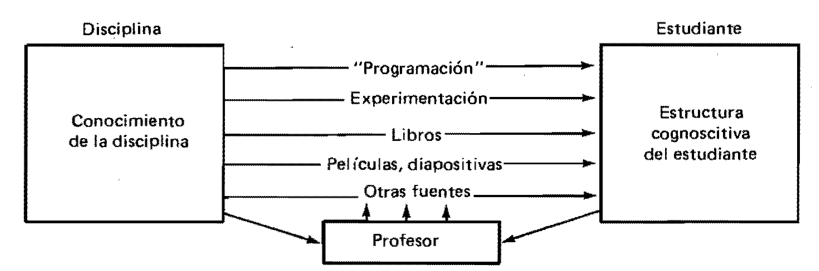
\includegraphics[width = 0.6\linewidth]{Esquema.png}
    \caption{Modelo de planificación de enseñanza.}
    \label{fig:esq}
\end{figure}

Por el cual recordé el ensayo de la lección 3. Ya que justamente se plantea un sistema de enseñanza donde el profesor se encarga de preparar el material para que el alumno cree su propio aprendizaje, y el profesor aparece como una guía extra y no el único (ni el principal) camino para el aprendizaje del estudiante.

Además dentro del modelo se consideran los distintos materiales didácticos que pueden ser utilizados. Estos se relacionan con la parte del modelo que habla del contexto y la cultura disponible. Ya que dentro de esa cultura se pueden utilizar ejemplos con aplicaciones directas, u otros recursos que ayuden con el aprendizaje, la formación de conexiones y el interés del estudiante. Como lo son los laboratorios, materiales impresos, auxiliares didácticos, películas y televisión entre otros recursos.

Finalmente se toca otro tema muy importante, establecer los objetivos del aprendizaje. Esto es una clara ayuda tanto para el estudiante como para el maestro, ya que el estudiante tiene los ojos fijos en la meta, es como darle un mapa y marcar con una $X$ el destino, aunque después lo vayas guiando por la ruta correcta. Y en el caso del profesor, ayuda a plantearse clases realistas, pero que a la vez abarquen un poco más del objetivo para asegurar que al menos este se cumpla.